% ERD database NADI, sesuai prototipe-ui/JunproProject/Database/schema.sql
% Kompilasi: pdflatex erd.tex
\documentclass[border=12pt]{standalone}
\usepackage[T1]{fontenc}
\usepackage{lmodern}
\usepackage{tikz}
\usepackage{array}
\usetikzlibrary{positioning,calc}

\renewcommand{\familydefault}{\sfdefault}

% Satu entitas = judul + daftar atribut (PK/FK di kolom kiri).
\newcommand{\entitas}[2]{%
  \begin{tabular}{@{}>{\footnotesize}l@{\hspace{6pt}}l@{\hspace{10pt}}>{\footnotesize\itshape}l@{}}
    \multicolumn{3}{@{}c@{}}{\textbf{#1}}\\[2pt]\hline\noalign{\vspace{2pt}}
    #2
  \end{tabular}}

\begin{document}
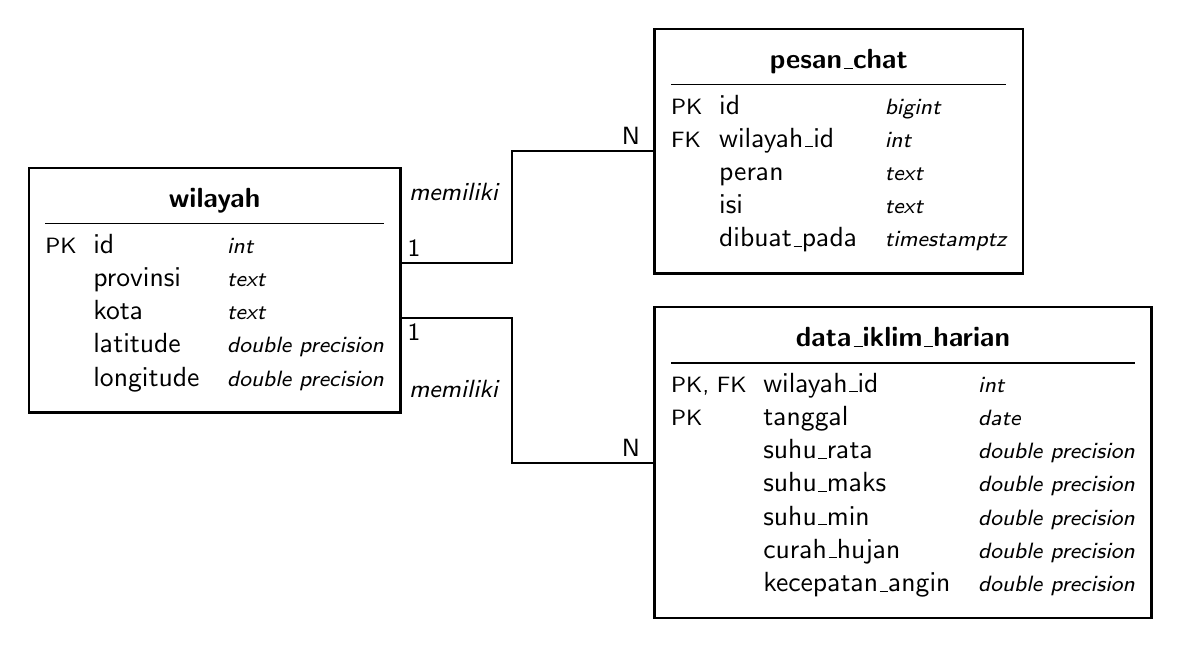
\begin{tikzpicture}[
    tabel/.style={draw, thick, inner sep=6pt, fill=white},
    relasi/.style={thick},
    kardinal/.style={font=\small, inner sep=2pt}
  ]

  \node[tabel] (wilayah) {\entitas{wilayah}{
    PK & id         & int \\
       & provinsi   & text \\
       & kota       & text \\
       & latitude   & double precision \\
       & longitude  & double precision \\
  }};

  \node[tabel, above right=0.2cm and 3.2cm of wilayah.east, anchor=south west] (chat) {\entitas{pesan\_chat}{
    PK & id          & bigint \\
    FK & wilayah\_id & int \\
       & peran       & text \\
       & isi         & text \\
       & dibuat\_pada & timestamptz \\
  }};

  \node[tabel, below right=0.2cm and 3.2cm of wilayah.east, anchor=north west] (iklim) {\entitas{data\_iklim\_harian}{
    PK, FK & wilayah\_id     & int \\
    PK     & tanggal         & date \\
           & suhu\_rata      & double precision \\
           & suhu\_maks      & double precision \\
           & suhu\_min       & double precision \\
           & curah\_hujan    & double precision \\
           & kecepatan\_angin & double precision \\
  }};

  % wilayah 1 --- N pesan_chat
  \coordinate (a) at ($(wilayah.east)+(0,0.35)$);
  \draw[relasi] (a) -- ++(1.4,0) |- (chat.west)
    node[kardinal, pos=0.92, above] {N};
  \node[kardinal, above right] at (a) {1};
  \node[font=\small\itshape, anchor=east] at ($(a)+(1.35,0.9)$) {memiliki};

  % wilayah 1 --- N data_iklim_harian
  \coordinate (b) at ($(wilayah.east)+(0,-0.35)$);
  \draw[relasi] (b) -- ++(1.4,0) |- (iklim.west)
    node[kardinal, pos=0.92, above] {N};
  \node[kardinal, below right] at (b) {1};
  \node[font=\small\itshape, anchor=east] at ($(b)+(1.35,-0.9)$) {memiliki};

\end{tikzpicture}
\end{document}
